\section{User Effects}
% Illustration of setup/positions on slide 1
% One slide for each:
    % All S11 on slide 2 
    % All S22 on slide 3
    % All S21 on slide 4
    % All efficiency on slide 5
    % All correlation on slide 6
    % All SAR on slide 7 (only one figure)
% For each slide, three figures/subplot (for each design)
    % Blue (freespace[0]), alpha 0.5 (min(freespace))
    % Green (data[0]), alpha 0.5 (min(data))
    % Red (play[0]), alpha 0.5 (min(play))
    % Cyan (talk[0]), alpha 0.5 (min(talk))

\def\legendfooter{\scriptsize{(1) Monopole (2) Triangle-feed (3) Dual-feed. \textcolor{bb}{Free-space}, \textcolor{gg}{Data}, \textcolor{rr}{Play}, \textcolor{cc}{Talk}. Frequency in MHz.}}
\def\emptyline{\textcolor{white}{Empty}}
\begin{frame}
    \frametitle{User Effects}
    Now comes a lot of plots\ldots

    Stick with me!
\end{frame}

\begin{frame}
    \frametitle{User Effects -- S11, minimum over tunable range}
    % \emptyline
    Design 2 is generally is better matched.
    \begin{center}
        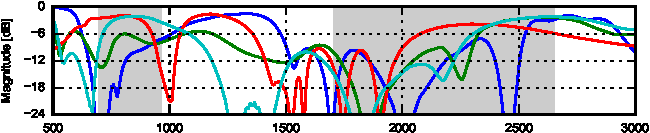
\includegraphics{img/soren/ue/design1lt/s11top.pdf}\\
        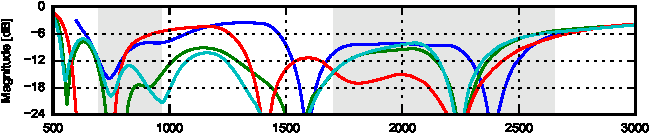
\includegraphics{img/soren/ue/design2sn/s11top.pdf}\\
        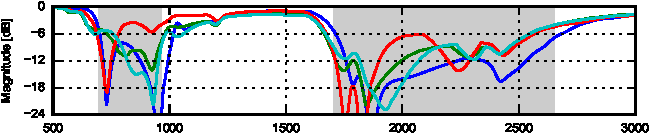
\includegraphics{img/soren/ue/design3hv/s11top.pdf}
    \end{center}
    \legendfooter
\end{frame}

\begin{frame}
    \frametitle{User Effects -- S22, minimum over tunable range}
    % \emptyline
    Detuning. Design 2 is better matched.
    \begin{center}
        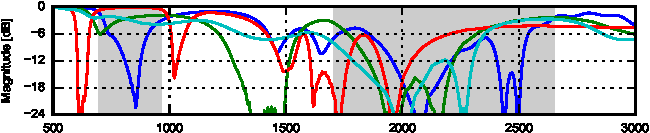
\includegraphics{img/soren/ue/design1lt/s22side.pdf}\\
        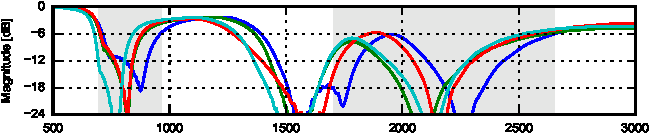
\includegraphics{img/soren/ue/design2sn/s22side.pdf}\\
        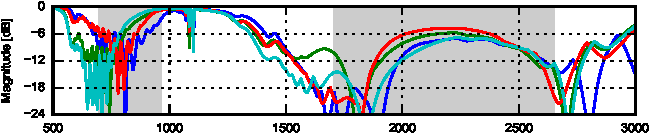
\includegraphics{img/soren/ue/design3hv/s22side.pdf}
    \end{center}
    \legendfooter
\end{frame}

\begin{frame}
    \frametitle{User Effects -- Total efficiency, minimum over tunable range (top)}
    % \emptyline
    Design 2 and 3 is better.
    \begin{center}
        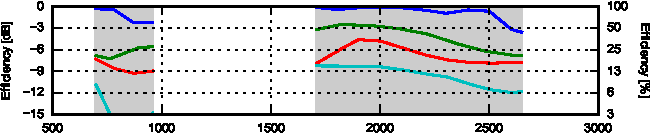
\includegraphics{img/soren/ue/design1lt/efftop.pdf}\\
        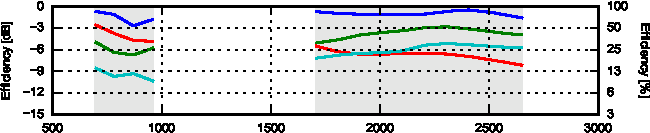
\includegraphics{img/soren/ue/design2sn/efftop.pdf}\\
        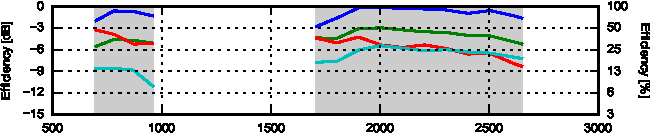
\includegraphics{img/soren/ue/design3hv/efftop.pdf}
    \end{center}
    \legendfooter
\end{frame}

\begin{frame}
    \frametitle{User Effects -- Total efficiency, minimum over tunable range (side)}
    % \emptyline
    Design 2 is better.
    \begin{center}
        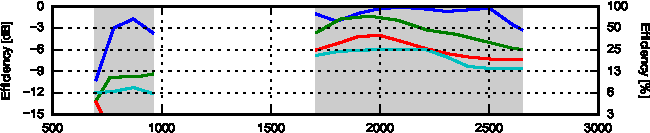
\includegraphics{img/soren/ue/design1lt/effside.pdf}\\
        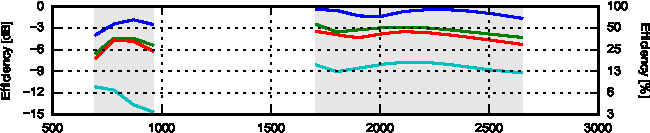
\includegraphics{img/soren/ue/design2sn/effside.pdf}\\
        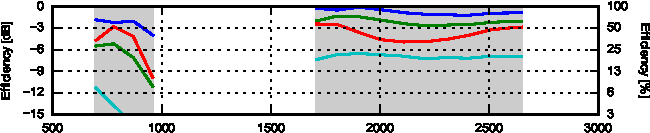
\includegraphics{img/soren/ue/design3hv/effside.pdf}
    \end{center}
    \legendfooter
\end{frame}

\begin{frame}
    \frametitle{User Effects -- Correlation, minimum over tunable range (tuning top)}
    Increase and decrease in correlation for different use cases.
    \emptyline
    \begin{center}
        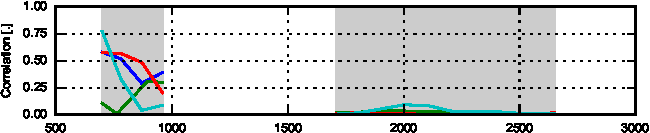
\includegraphics{img/soren/ue/design1lt/corrtop.pdf}\\
        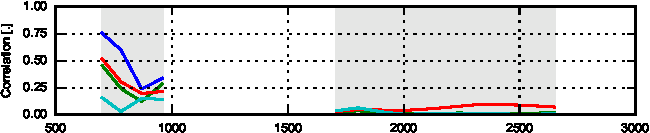
\includegraphics{img/soren/ue/design2sn/corrtop.pdf}\\
        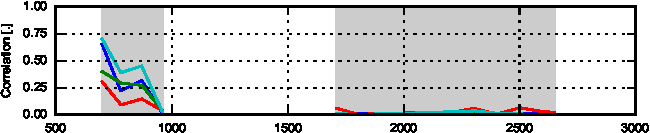
\includegraphics{img/soren/ue/design3hv/corrtop.pdf}
    \end{center}
    \legendfooter
\end{frame}

\begin{frame}
    \frametitle{User Effects -- Correlation, minimum over tunable range (tuning side)}
    Increase and decrease in correlation for different use cases.
    \emptyline
    \begin{center}
        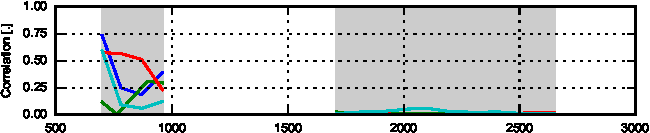
\includegraphics{img/soren/ue/design1lt/corrside.pdf}\\
        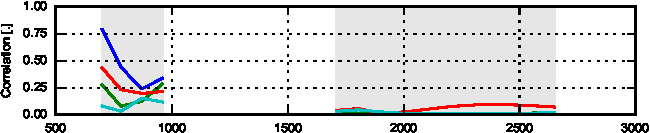
\includegraphics{img/soren/ue/design2sn/corrside.pdf}\\
        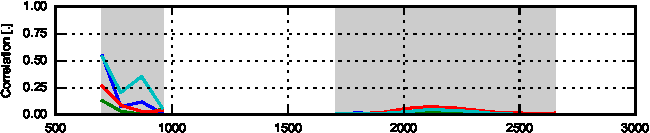
\includegraphics{img/soren/ue/design3hv/corrside.pdf}
    \end{center}
    \legendfooter
\end{frame}

\section{Prototypes}
\begin{frame}
    \frametitle{Prototypes}
    Images of prototypes
\end{frame}

\def\legendfooter{\scriptsize{Upper: Top antenna. Lower: Side antenna. Frequency in MHz.}}
\begin{frame}
    \frametitle{Prototype 1 -- Monopole}
    \emptyline
    \begin{center}
        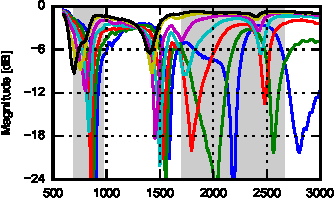
\includegraphics{img/soren/proto/design1lt/s11.pdf}
        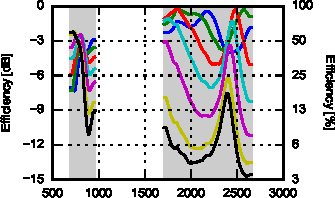
\includegraphics{img/soren/proto/design1lt/efftop.pdf}\\
        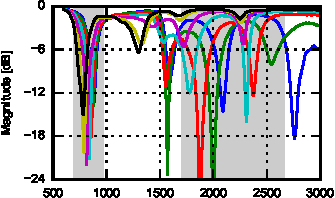
\includegraphics{img/soren/proto/design1lt/s22.pdf}
        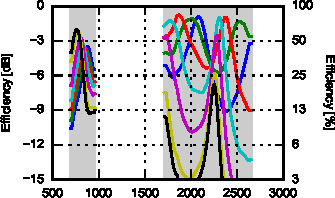
\includegraphics{img/soren/proto/design1lt/effside.pdf}
    \end{center}
    \legendfooter
\end{frame}

\begin{frame}
    \frametitle{Prototype 2 -- Triangle-feed}
    \emptyline
    \begin{center}
        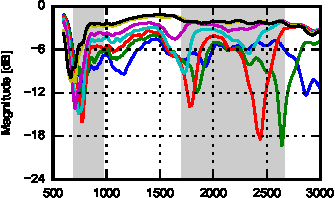
\includegraphics{img/soren/proto/design2sn/s11.pdf}
        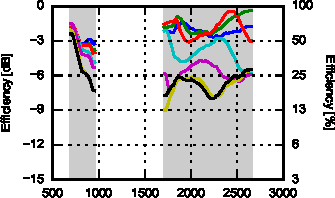
\includegraphics{img/soren/proto/design2sn/efftop.pdf}\\
        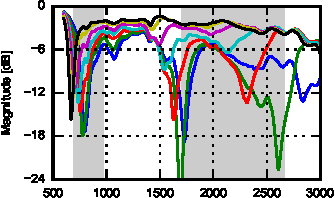
\includegraphics{img/soren/proto/design2sn/s22.pdf}
        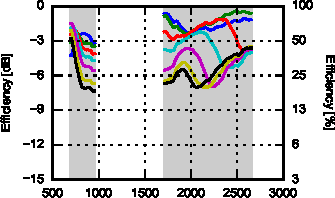
\includegraphics{img/soren/proto/design2sn/effside.pdf}
    \end{center}
    \legendfooter
\end{frame}

\begin{frame}
    \frametitle{Prototype 3 -- Dual-feed}
    \emptyline
    \begin{center}
        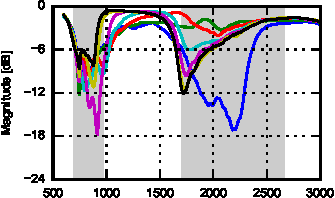
\includegraphics{img/soren/proto/design3hv/s11.pdf}
        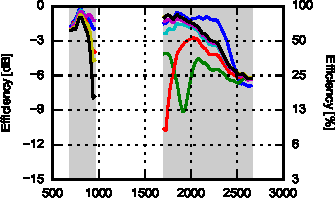
\includegraphics{img/soren/proto/design3hv/efftop.pdf}\\
        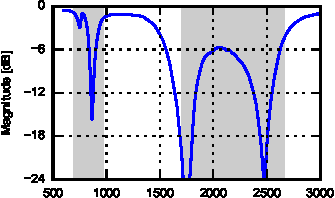
\includegraphics{img/soren/proto/design3hv/s22.pdf}
        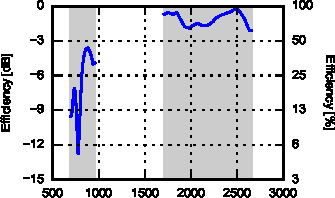
\includegraphics{img/soren/proto/design3hv/effside.pdf}
    \end{center}
    \legendfooter
\end{frame}

\begin{frame}
    \frametitle{Preliminary Conclusion}
\end{frame}
